\chapter{Tableaux semânticos na lógica de predicados}


Capítulo 13 de Souza, \textit{Lógica para Ciência da Computação}~\cite{souza_logica_1}.

\vspace{1cm}


%%%%%%%%%%%%%%%%%%%%
\begin{easylist}
  & Elementos do sistema de tableaux semânticos da lógica de predicados:
  && Alfabeto da lógica de predicados
  && Conjunto das fórmulas da lógica de predicados
  && Um conjunto de regras de dedução

  \SKIP
  & Regras de dedução do tableau semântico: sejam $A$ e $B$ duas fórmulas da lógica de predicados, as regras $R_1$ a $R_9$ são as mesmas do sistema de tableaux semânticos da lógica de predicados. As demais são

\begin{figure}[h!]
  \begin{center}
    \begin{tabular}{c}
      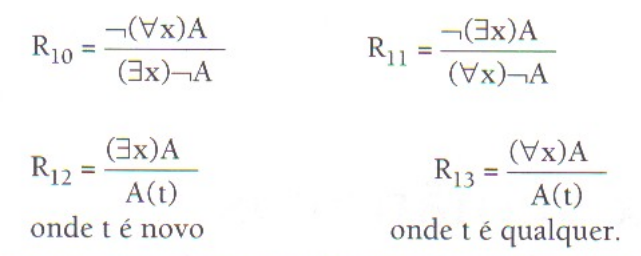
\includegraphics[width=0.7\textwidth]{images/13/tableaux.png}
    \end{tabular}
  \end{center}
  %\caption{\label{fig:tree:01}}
\end{figure}

\clearpage
&& Exemplo: mostre que a fórmula $H = (\FA x)(\FA y)p(x, y) \IMP p(a, a))$ é tautologia.

\end{easylist}
\begin{prooftree}
  {
    to prove={(\FA x)(\FA y)p(x, y) \IMP p(a, a))}
  }
  [{    \NOT(  (\FA x)(\FA y)p(x, y) \IMP p(a, a)  )    }, just={$\NOT H$}, checked
    [{    (\FA x)(\FA y)p(x, y)    }, just={$R_8$ em 1}, checked
      [{    \NOT p(a, a)    }, just={$R_8$ em 1}
        [{    (\FA y)p(a, y)    }, just={$R_{13}$ em 2, $x=a$}, checked
          [{    p(a, a)    }, just={$R_{13}$ em 4, $y=a$}, close={5,3}
          ]
        ]
      ]
    ]
  ]
\end{prooftree}

%%%%%%%%%%%%%%%%%%%%%%%%%%%%%%%%%%%%%%%%
\begin{easylist}

\SKIP
&& Exemplo: mostre que a fórmula $H = (\FA x)p(x) \IMP (\EX y)p(y)$ é tautologia.

\end{easylist}
\begin{prooftree}
  {
    to prove={(\FA x)p(x) \IMP (\EX y)p(y)}
  }
  [{    \NOT(  (\FA x)p(x) \IMP (\EX y)p(y)  )    }, just={$\NOT H$}, checked
    [{    (\FA x)p(x)    }, just={$R_8$ em 1}, checked
      [{    \NOT (\EX y)p(y)    }, just={$R_8$ em 1}, checked
        [{    (\FA y)\NOT p(y)    }, just={$R_{11}$ em 3}, checked
          [{    \NOT p(a)    }, just={$R_{13}$ em 4, $y=a$}
            [{    p(a)    }, just={$R_{13}$ em 2, $x=a$}, close={5,6}
            ]
          ]
        ]
      ]
    ]
  ]
\end{prooftree}


%%%%%%%%%%%%%%%%%%%%%%%%%%%%%%%%%%%%%%%%
\begin{easylist}

\SKIP
&& Exemplo: mostre que a fórmula $H = (\EX x)(\EX y)p(x, y) \IMP p(a, a))$ é tautologia.

\end{easylist}
\begin{prooftree}
  {
    to prove={(\EX x)(\EX y)p(x, y) \IMP p(a, a))}
  }
  [{    \NOT(  (\EX x)(\EX y)p(x, y) \IMP p(a, a)  )    }, just={$\NOT H$}, checked
    [{    (\EX x)(\EX y)p(x, y)    }, just={$R_8$ em 1}, checked
      [{    \NOT p(a, a)    }, just={$R_8$ em 1}
        [{    (\EX y)p(b_1, y)    }, just={$R_{13}$ em 2, $x=b_1$}, checked
          [{    p(b_1, b_2)    }, just={$R_{13}$ em 4, $y=b_2$}
          ]
        ]
      ]
    ]
  ]
\end{prooftree}

O tableau não pode ser fechado, então $H$ não é tautologia.

%%%%%%%%%%%%%%%%%%%%%%%%%%%%%%%%%%%%%%%%
\begin{easylist}

\clearpage
& Teorema no sistema de tableaux semânticos da lógica de predicados.
&& Considere o teorema $H = (\FA x)(p(x) \AND q(x)) \IMP (\FA x)P(x)$. O tableau abaixo mostra que $\ISINT H$.

\end{easylist}
\begin{prooftree}
  {
    to prove={(\FA x)(p(x) \AND q(x)) \IMP (\FA x)p(x)}
  }
  [{    \NOT(  (\FA x)(p(x) \AND q(x)) \IMP (\FA x)p(x)  )    }, just={$\NOT H$}, checked
    [{    (\FA x)(p(x) \AND q(x))    }, just={$R_8$ em 1}, checked
      [{    \NOT(\FA x)P(x)    }, just={$R_8$ em 1}, checked
        [{    (\EX x)\NOT p(x)    }, just={$R_{10}$ em 3}, checked
          [{    \NOT p(a)    }, just={$R_{12}$ em 3, $x=a$}
            [{    p(a) \AND q(a)    }, just={$R_{13}$ em 2, $x=a$}, checked
              [{    p(a)    }, just={$R_1$ em 6}
                [{    q(a)    }, just={$R_1$ em 6}, close={5,7}
                ]
              ]
            ]
          ]
        ]
      ]
    ]
  ]
\end{prooftree}
  
%%%%%%%%%%%%%%%%%%%%%%%%%%%%%%%%%%%%%%%%
\begin{easylist}

&& O tableau abaixo porém, onde a aplicação das regras é invertida, não é fechado.

\end{easylist}
\begin{prooftree}
  {
    to prove={(\FA x)(p(x) \AND q(x)) \IMP (\FA x)p(x)}
  }
  [{    \NOT(  (\FA x)(p(x) \AND q(x)) \IMP (\FA x)p(x)  )    }, just={$\NOT H$}, checked
    [{    (\FA x)(p(x) \AND q(x))    }, just={$R_8$ em 1}, checked
      [{    \NOT(\FA x)P(x)    }, just={$R_8$ em 1}, checked
        [{    (\EX x)\NOT p(x)    }, just={$R_{10}$ em 3}, checked
          [{    p(a) \AND q(a)    }, just={$R_{13}$ em 2, $x=a$}, checked
            [{    p(a)    }, just={$R_1$ em 5}
              [{    q(a)    }, just={$R_1$ em 5}
                [{    \NOT p(b)    }, just={$R_{12}$ em 4, $x=b$}
                ]
              ]
            ]
          ]
        ]
      ]
    ]
  ]
\end{prooftree}

%%%%%%%%%%%%%%%%%%%%%%%%%%%%%%%%%%%%%%%%
\begin{easylist}

  \SKIP
  && Ao desenvolver um tableau, priorize sempre a aplicação de $R_{12}$ em detrimento de $R_{13}$. Assim o termo usado na aplicação de $R_{13}$ pode ser o mesmo usado na aplicação de $R_{12}$, facilitando a repetição de fórmulas necessária para fechar os ramos do tableau.
  \SKIP
  && Podemos afirmar o seguinte sobre tableaux semânticos associados a fórmulas da lógica de predicados.
  &&& Se $H$ é tautologia, então existe tableau fechado associado a $H$.
  &&& Se $H$ é tautologia, então pode existir tableau aberto associado a $H$.
  &&& Se $H$ não é tautologia, então todo tableau associado a $H$ é aberto.
  &&& Se um tableau associado a $H$ é fechado, então $H$ é tautologia.
  &&& Se um tableau associado a $H$ é aberto, então não se pode concluir que $H$ não é tautologia.
  &&& Se todo tableau associado a $H$ é aberto, então $H$ não é tautologia.
  
\end{easylist}

%%%%%%%%%%%%%%%%%%%%%%%%%%%%%%%%%%%%%%%%
\clearpage
\newgeometry{left=0.1cm}
\begin{easylist}

  & Consequência lógica em tableaux semânticos:
  && Sejam $H_1$ e $H_2$ duas fórmulas da lógica de predicados. Dizemos que $H_1$ equivale a $H_2$ se e somente se $H_1 \BIC H_2$ é tautologia.
  \SKIP
  && Exemplo: sejam $H_1 = (\EX x)(p(x) \IMP q(x))$ e $H_2 = (\FA x)p(x) \IMP (\EX x)q(x)$. Mostre que $H_1$ equivale a $H_2$.

\tiny
\end{easylist}
\begin{prooftree}
  {
    to prove={(\EX x)(p(x) \IMP q(x)) \BIC ((\FA x)p(x) \IMP (\EX x)q(x))}
  }
  [{    \NOT(  (\EX x)(p(x) \IMP q(x)) \BIC ((\FA x)p(x) \IMP (\EX x)q(x))  )    }, just={$\NOT(H_1 \BIC H_2)$}, checked
    [{    (\EX x)(p(x) \IMP q(x)) \AND \NOT((\FA x)p(x) \IMP (\EX x)q(x))    }, just={$R_9$ em 1}, checked
      [{    (\EX x)(p(x) \IMP q(x))    }, just={$R_1$ em 2}, checked
        [{    \NOT((\FA x)p(x) \IMP (\EX x)q(x))    }, just={$R_1$ em 2}, checked
          [{    (\FA x)p(x)    }, just={$R_8$ em 4}, checked
            [{    \NOT(\EX x)q(x)    }, just={$R_8$ em 4}, checked
              [{    (\FA x)\NOT q(x)    }, just={$R_{11}$ em 6}, checked
                [{    (p(a) \IMP q(a))    }, just={$R_{12}$ em 3, $x=a$}, checked
                  [{    p(a)    }, just={$R_{13}$ em 5, $x=a$}
                    [{    \NOT q(a)    }, just={$R_{13}$ em 7, $x=a$}
                      [{    \NOT p(a)    }, just={$R_3$ em 8}, close={9,11}]
                      [{    q(a)    }, just={$R_3$ em 8}, close={10,11}]
                    ]
                  ]
                ]
              ]
            ]
          ]
        ]
      ]
    ]
    [{    \NOT(\EX x)(p(x) \IMP q(x)) \AND ((\FA x)p(x) \IMP (\EX x)q(x))    }, just={$R_9$ em 1}, checked
      [{    \NOT(\EX x)(p(x) \IMP q(x))    }, just={$R_1$ em 2}, checked
        [{    ((\FA x)p(x) \IMP (\EX x)q(x))    }, just={$R_1$ em 2}, checked
          [
            [
              [
                [
                  [
                    [
                      []
                      [
                        [{    (\FA x)\NOT(p(x) \IMP q(x))    }, just={$R_{11}$ em 3}, checked
                          [{    \NOT(\FA x)p(x)    }, just={$R_3$ em 4}, checked
                            [{    (\EX x)\NOT p(x)    }, just={$R_{10}$ em 13}, checked
                              [{    \NOT p(a)    }, just={$R_{12}$ em 14}
                                [{    \NOT(p(a) \IMP q(a))    }, just={$R_{13}$ em 12, $x=a$}, checked
                                  [{    p(a)    }, just={$R_8$ em 16}
                                    [{    \NOT q(a)    }, just={$R_8$ em 16}, close={15,17}
                                    ]
                                  ]
                                ]
                              ]
                            ]
                          ]
                          [{    (\EX x)q(x)    }, just={$R_3$ em 4}, checked
                            [
                              [{    q(a)    }, just={$R_{12}$ em 13, $x=a$}
                                [{    \NOT(p(a) \IMP q(a))    }, just={$R_{13}$ em 12, $x=a$}, checked
                                  [{    p(a)    }, just={$R_8$ em 16}
                                    [{    \NOT q(a)    }, just={$R_8$ em 16}, close={15,18}
                                    ]
                                  ]
                                ]
                              ]
                            ]
                          ]
                        ]
                      ]
                    ]
                  ]
                ]
              ]
            ]
          ]
        ]
      ]
    ]
  ]
\end{prooftree}
\restoregeometry

%%%%%%%%%%%%%%%%%%%%%%%%%%%%%%%%%%%%%%%%
\clearpage
\begin{easylist}

  && Sejam $H_1$ e $H_2$ duas fórmulas da lógica de predicados. Dizemos que $H_1$ implica em $H_2$ se e somente se $H_1 \IMP H_2$ é tautologia.
  \SKIP
  && Exemplo: sejam $H_1 = (\FA x)(p(x) \IMP q(x))$ e $H_2 = (\EX x)p(x) \IMP (\FA x)q(x)$. Mostre que $H_2$ implica em $H_1$.

\tiny
\end{easylist}
\begin{prooftree}
  {
    to prove={((\EX x)p(x) \IMP (\FA x)q(x)) \IMP (\FA x)(p(x) \IMP q(x))}
  }
  [{    \NOT(  ((\EX x)p(x) \IMP (\FA x)q(x)) \IMP (\FA x)(p(x) \IMP q(x))  )    }, just={$\NOT(H_1 \BIC H_2)$}, checked
    [{    (\EX x)p(x) \IMP (\FA x)q(x)    }, just={$R_{8}$ em 1}, checked
      [{    \NOT(\FA x)(p(x) \IMP q(x))    }, just={$R_{8}$ em 1}, checked
        [{    (\EX x)\NOT(p(x) \IMP q(x))    }, just={$R_{10}$ em 3}, checked
          [{    \NOT(p(a) \IMP q(a))    }, just={$R_{12}$ em 4, $x=a$}, checked
            [{    p(a)    }, just={$R_{8}$ em 5}, checked
              [{    \NOT q(a)    }, just={$R_{8}$ em 5}, checked
                [{    \NOT(\EX x)p(x)    }, just={$R_{9}$ em 2}, checked
                  [{    (\FA x)\NOT p(x)    }, just={$R_{12}$ em 8}, checked
                    [{    \NOT p(a)    }, just={$R_{13}$ em 8}, close={6,10}
                    ]
                  ]
                ]
                [{    (\FA x)q(x)    }, just={$R_{9}$ em 2}, checked
                  [
                    [{    q(a)    }, just={$R_{13}$ em 9, $x=a$}, close={7,10}
                    ]
                  ]
                ]
              ]
            ]
          ]
        ]
      ]
    ]
  ]
\end{prooftree}



%%%%%%%%%%%%%%%%%%%%%%%%%%%%%%%%%%%%%%%%%%%%%%%%%%%%%%%%%%%%
\section{Exercícios}

%$ \NOT \; \OR \; \AND \; \IMP \; \BIC$

\begin{enumerate}
  \item Determine se as fórmulas a seguir são ou não equivalentes usando o método dos tableaux semânticos.
    \begin{enumerate}
      \item $(\FA x)q(y)$ e $q(y)$
      \item $(\EX x)q(y)$ e $q(y)$
      \item $(\FA x)(p(x) \AND q(y))$ e $(\FA x)(p(x) \AND q(y)$
      \item $(\EX x)(p(x) \AND q(y))$ e $(\EX x)(p(x) \AND q(y)$
      \item $(\FA x)(p(x) \OR q(y))$ e $(\FA x)(p(x) \OR q(y)$
      \item $(\EX x)(p(x) \OR q(y))$ e $(\EX x)(p(x) \OR q(y)$
      \item $(\FA x)(p(x) \IMP q(y))$ e $(\FA x)(p(x) \IMP q(y)$
      \item $(\EX x)(p(x) \IMP q(y))$ e $(\EX x)(p(x) \IMP q(y)$
    \end{enumerate}
\end{enumerate}
